%\section*{ Introduction to Repeated Two-person Zero-Sum Games}

%\markright{Rock-Paper-Scissors}
\section{Mixed Strategies: Linear Solution}

Let's continue to consider the game given by $\left[\begin{matrix}
1&0\\
-1&2

\end{matrix}\right].$

In order to make our analysis easier, let's name the row and column strategies:

\begin{tabular}{rcc}
&\textbf{C}&\textbf{D}\\ 
\textbf{A} &1&0 \\ 
\textbf{B}&-1&2 \\ 
\end{tabular}.

We want to determine how often Player 1 should play A and how often she should play B. First it is good to test your instinct. Do you think she should play one of the strategies more often than the other? 
%[It should seem like she should play A more than B.] 
What we are really trying to find is the probability with which Player 1 plays A (or B). Since we know that the probabilities sum to one, if we can find one probability, then we know the other. 

Here is one way to do this. Let $p$ be the probability that Player 1 plays B. Let $m$ be the payoff to Player 1. Since we are try to find a mixed strategy for Player 1, we will pick a strategy for Player 2 and try to determine the possible payoffs for Player 1.

 Let us determine some pairs $(p, m)$.
\begin{itemize}
\item Step 1. Assume {\bf Player 2} plays pure strategy {\bf C}.
\begin{enumerate}
\item If Player 1 plays pure strategy {\bf A}, then she never plays {\bf B}. Thus the probability she play B is 0. Hence,  $p=0$. In the case where Player 1 plays {\bf A} and Player 2 play {\bf C}, what is the payoff to Player 1? This is $m$, so $m=1$. Thus, for the strategy pair $\{A, C\}$ we get $(0, 1)$ for $(p, m)$. It is important to note that $(0, 1)$ is {\it not} a payoff vector. This is common notation for any ordered pair. WIth payoff vectors, the ordered pair represents the payoff to each player. Here the ordered pair represents a probability of playing B and the payoff to Player 1.
\item If Player 1 plays pure strategy {\bf B}, then what is the probability that she plays B? $p=1$. What is the payoff to Player 1? $m=-1$. Thus, for the strategy pair $\{B, C\}$ we get $(1, -1)$ for $(p, m)$.
\item Now we want to know what Player 1's payoff will be as she varies the probability, $p$, with which she plays B. We can draw a graph where the $x$-axis represents to probability with which she plays $B$ and the $y$-axis represents the expected payoff.

%\begin{figure}[h]
%\leavevmode
%\begin{center}
%{\scalebox{.65}{\input{graph1.pstex_t}}}
%\end{center}
%\end{figure}  

\begin{figure}
\begin{center}
\begin{tikzpicture}
\begin{axis}[axis lines=middle, xmin=-0.25,xmax=1.4, ymin=-1.5, ymax=2.5,xtick={0,1},ytick={0,0}]
%\addplot[-, mark=*]coordinates{(0,0)(1,2)}
%node[pos=0,above left]{$(0,0)$}
%node[pos=1,above]{$(1,2)$}
%node[pos=.5,above]{$D$};

%\addplot[-, mark=*]coordinates{(0,1)(1,-1)}
%node[pos=0,above left]{$(0,1)$}
%node[pos=1,above right]{$(1,-1)$}
%node[pos=.7,below]{$C$};

\node[anchor=south west]
at ({axis cs:0,0}|-{axis description cs: 0,0}){$A$};

\node[anchor=south west]
at ({axis cs:1,0}|-{axis description cs: 0,0}){$B$};

\end{axis}
\end{tikzpicture}
\captionof{figure}{Mixed Strategy Axes}
   \label{MixedStrategyAxes}
\end{center}   
\end{figure}


Thus, when Player 1 plays only A, she is playing B with probability 0; when Player 1 plays only B, she is playing B with probability 1. It might be easier to remember if you label your graph as above.
\item Now we can plot the points we determined in (1) and (2). We will connect them with a line representing Player 2's pure strategy C.

%\begin{figure}[h]
%\leavevmode
%\begin{center}
%{\scalebox{.65}{\input{graph2.pstex_t}}}
%\end{center}
%\end{figure}  

\begin{figure}
\begin{center}
\begin{tikzpicture}
\begin{axis}[axis lines=middle, xmin=-0.25,xmax=1.4, ymin=-1.5, ymax=2.5,xtick={0,1}]
%\addplot[-, mark=*]coordinates{(0,0)(1,2)}
%node[pos=0,above left]{$(0,0)$}
%node[pos=1,above]{$(1,2)$}
%node[pos=.5,above]{$D$};

\addplot[-, mark=*]coordinates{(0,1)(1,-1)}
node[pos=0,above left]{$(0,1)$}
node[pos=1,above right]{$(1,-1)$}
node[pos=.7,below]{$C$};

\node[anchor=south west]
at ({axis cs:0,0}|-{axis description cs: 0,0}){$A$};

\node[anchor=south west]
at ({axis cs:1,0}|-{axis description cs: 0,0}){$B$};

\end{axis}
\end{tikzpicture}
\captionof{figure}{Player 2's pure strategy $C$}
   \label{MixedStrategyOneLine}
\end{center}
\end{figure}


Before moving on, let's make sure we understand what this line represents. Any point on it represents the expected payoff to Player 1 as she varies her strategy, {\it assuming Player 2 only plays C}. In this case, we can see that as she plays B more often, her expected payoff goes down. 
\end{enumerate}

Now let's do the same thing, assuming Player 2 plays only D.
\item  Step 2. Assume {\bf Player 2} plays pure strategy {\bf D}.
\begin{enumerate}
\item If Player 1 plays pure strategy {\bf A}, then what is the probability that she plays B? $p=0$. What is the payoff to Player 1? $m=0$. Thus, for the strategy pair $\{A, D\}$ we get $(0, 0)$ for $(p, m)$.
\item If Player 1 plays pure strategy {\bf B}, then what is the probability that she plays B? $p=1$. What is the payoff to Player 1? $m=2$. Thus, for the strategy pair $\{B, D\}$ we get $(1, -1)$ for $(p, m)$.
\item Now, on our same graph from Step 1, we can plot the points we determined in (1) and (2). We will connect them with a line representing Player 2's pure strategy D.

%\begin{figure}[h]
%\leavevmode
%\begin{center}
%{\scalebox{.65}{\input{graph3.pstex_t}}}
%\end{center}
%\end{figure}  

\begin{figure}
\begin{center}
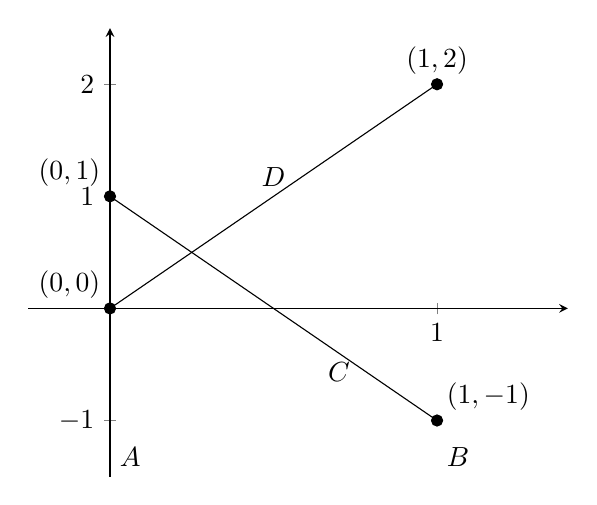
\begin{tikzpicture}
\begin{axis}[axis lines=middle, xmin=-0.25,xmax=1.4, ymin=-1.5, ymax=2.5,xtick={0,1}]
\addplot[-, mark=*]coordinates{(0,0)(1,2)}
node[pos=0,above left]{$(0,0)$}
node[pos=1,above]{$(1,2)$}
node[pos=.5,above]{$D$};

\addplot[-, mark=*]coordinates{(0,1)(1,-1)}
node[pos=0,above left]{$(0,1)$}
node[pos=1,above right]{$(1,-1)$}
node[pos=.7,below]{$C$};

\node[anchor=south west]
at ({axis cs:0,0}|-{axis description cs: 0,0}){$A$};

\node[anchor=south west]
at ({axis cs:1,0}|-{axis description cs: 0,0}){$B$};

\end{axis}
\end{tikzpicture}
\captionof{figure}{Mixed Strategy Two Lines}
   \label{Player 2's pure strategy $D$}
\end{center}   
\end{figure}

Now we can see that if Player 2 plays only D, then Player 1 does best by playing only B.
\end{enumerate}

\end{itemize}

So we have this nice graph, but what does it really tell us? Although we drew lines representing each of Player 2's pure strategies, Player 1 doesn't know what Player 2 will do. Suppose Player 1 only played A, while Player 2 plays an unknown mixed strategy. Then the possible payoffs for Player 1 are 1 or 0. The more often Player 2 plays C, the more often Player 1 gets 1. So the {\it expected payoff} per game for a repeated game varies between 0 and 1. We can see the possible expected values as the red line on the graph.

\break

%\begin{figure}[h]
%\leavevmode
%\begin{center}
%{\scalebox{.65}{\input{graph4.pstex_t}}}
%\end{center}
%\end{figure}  
\begin{figure}
\begin{center}
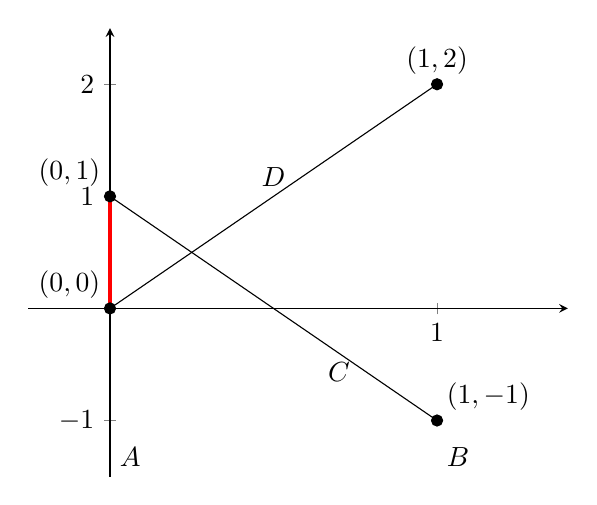
\begin{tikzpicture}
\begin{axis}[axis lines=middle, xmin=-0.25,xmax=1.4, ymin=-1.5, ymax=2.5,xtick={0,1}]
\addplot[-, mark=*]coordinates{(0,0)(1,2)}
node[pos=0,above left]{$(0,0)$}
node[pos=1,above]{$(1,2)$}
node[pos=.5,above]{$D$};

\addplot[-, mark=*]coordinates{(0,1)(1,-1)}
node[pos=0,above left]{$(0,1)$}
node[pos=1,above right]{$(1,-1)$}
node[pos=.7,below]{$C$};

\addplot[-, ultra thick, red]coordinates{(0,0)(0,1)};
%node[pos=0,above left]{$(0,1)$}
%node[pos=1,above right]{$(1,-1)$}
%node[pos=.7,below]{$C$};

\node[anchor=south west]
at ({axis cs:0,0}|-{axis description cs: 0,0}){$A$};

\node[anchor=south west]
at ({axis cs:1,0}|-{axis description cs: 0,0}){$B$};

\end{axis}
\end{tikzpicture}
\captionof{figure}{Possible expected value if Player 1 plays A}
   \label{BoldA}
\end{center}   
\end{figure}

Since we want to understand mixed strategies for Player 1, what would happen if Player 1 played A half the time and B half the time? In other words, what happens if $p=1/2$? Although we may not easily be able to see the exact values, we can represent the possible expected values on the graph. 

%\begin{figure}[h]
%\leavevmode
%\begin{center}
%{\scalebox{.65}{\input{graph5.pstex_t}}}
%\end{center}
%\end{figure}  

\begin{figure}
\begin{center}
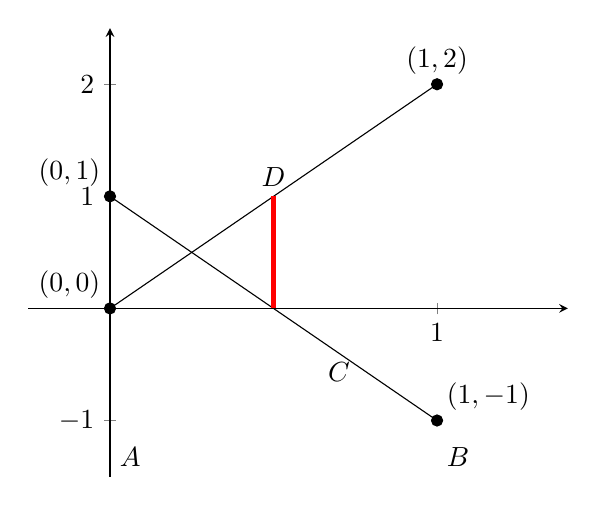
\begin{tikzpicture}
\begin{axis}[axis lines=middle, xmin=-0.25,xmax=1.4, ymin=-1.5, ymax=2.5,xtick={0,1}]
\addplot[-, mark=*]coordinates{(0,0)(1,2)}
node[pos=0,above left]{$(0,0)$}
node[pos=1,above]{$(1,2)$}
node[pos=.5,above]{$D$};

\addplot[-, mark=*]coordinates{(0,1)(1,-1)}
node[pos=0,above left]{$(0,1)$}
node[pos=1,above right]{$(1,-1)$}
node[pos=.7,below]{$C$};

\addplot[-, ultra thick, red]coordinates{(.5,0)(.5,1)};
%node[pos=0,above left]{$(0,1)$}
%node[pos=1,above right]{$(1,-1)$}
%node[pos=.7,below]{$C$};

\node[anchor=south west]
at ({axis cs:0,0}|-{axis description cs: 0,0}){$A$};

\node[anchor=south west]
at ({axis cs:1,0}|-{axis description cs: 0,0}){$B$};

\end{axis}
\end{tikzpicture}
\captionof{figure}{Player 1 plays B with probability 1/2}
   \label{BoldHalf}
\end{center}   
\end{figure}

Hopefully, you've begun to see that for each choice of $p$, the top line represents the highest expected value for Player 1; the bottom line represents the lowest expected value for Player 1; the area between the lines represents the possible expected values for Player 1. As we did with non-repeated games, let's look at the ``worst case scenario" for Player 1. In other words, let's assume that Player 2 can figure out Player 1's strategy. Then Player 1 would want to {\it maximize the minimum expected value}. Aha! This is just looking for the {\it maximin} stategy! 

Now the minimum expected value for each choice of $p$ is given by the bottom lines on the graph.

%\begin{figure}[h]
%\leavevmode
%\begin{center}
%{\scalebox{.65}{\input{graph6.pstex_t}}}
%\end{center}
%\end{figure}  

\begin{figure}
\begin{center}
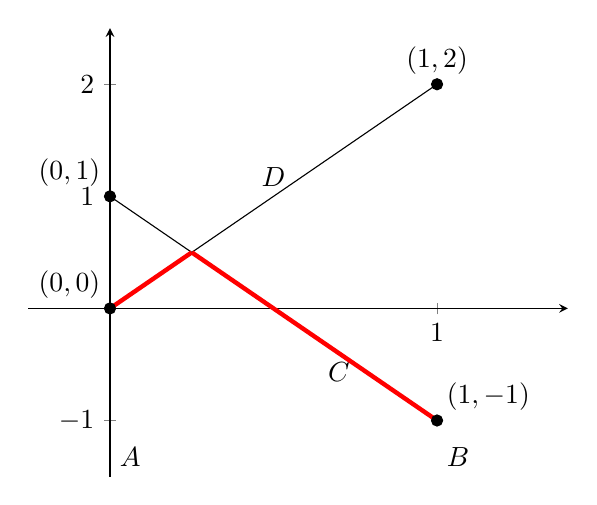
\begin{tikzpicture}
\begin{axis}[axis lines=middle, xmin=-0.25,xmax=1.4, ymin=-1.5, ymax=2.5,xtick={0,1}]
\addplot[-, mark=*]coordinates{(0,0)(1,2)}
node[pos=0,above left]{$(0,0)$}
node[pos=1,above]{$(1,2)$}
node[pos=.5,above]{$D$};

\addplot[-, mark=*]coordinates{(0,1)(1,-1)}
node[pos=0,above left]{$(0,1)$}
node[pos=1,above right]{$(1,-1)$}
node[pos=.7,below]{$C$};

\addplot[-, ultra thick, red]coordinates{(0,0)(.25,.5)};

\addplot[-, ultra thick, red]coordinates{(.25,.5)(1,-1)};
%node[pos=0,above left]{$(0,1)$}
%node[pos=1,above right]{$(1,-1)$}
%node[pos=.7,below]{$C$};

\node[anchor=south west]
at ({axis cs:0,0}|-{axis description cs: 0,0}){$A$};

\node[anchor=south west]
at ({axis cs:1,0}|-{axis description cs: 0,0}){$B$};

\end{axis}
\end{tikzpicture}
\captionof{figure}{Minimum Expected Payoff for Player 1}
   \label{BoldMin}
\end{center}      
\end{figure}

It should be easy to see that the {\it maximum} of the minimum expected payoffs occurs at the intersection of the two lines.

\begin{itemize}
\item Step 3. Find the intersection of the two lines.
\begin{enumerate}
\item Find the equation for Line C. This is the line passing through the points $(0, 1)$ and $(1, -1)$. It has slope $-2$ and $y$-intercept 1. Thus, it has equation $y=-2x+1$. [Although the $x$-axis represents probability $p$ and the $y$-axis represents expected payoff $m$, you are probably more comfortable solving equations--at least for the moment--in $x$ and $y$.]
\item Find the equation for Line D. This is the line passing through the points $(0, 0)$ and $(1, 2)$. It has slope $2$ and $y$-intercept 0. Thus, it has equation $y=2x$. 
\item Use substitution to find the point of intersection. 
\begin{eqnarray*}
2x &=&-2x+1\\
4x &=& 1\\
x&=&{1\over 4}
\end{eqnarray*}

Substituting $x={1\over 4}$ back in to either original equation, say $y=2x$, gives us $y={1\over 2}$. Thus, the point of intersection is $(1/4, 1/2)$. 
\end{enumerate}

\item Step 4. Determine Player 1's maximin mixed strategy. Recalling that the first coordinate is $p$, the probability that Player 1 plays {\it B}, we know that Player 1 will play B with probability 1/4, and thus, play A with probability 3/4 [$1-1/4=3/4$]. The expected payoff for Player 1 is 1/2. It is important to check back to your original intuition about the game. Did it seem as though Player 1 should play A more often than B?


\end{itemize}

Let's make a few important observations. First, it should be clear from the graph that Player 1 expects a payoff of 1/2 NO MATTER WHAT PLAYER 2 DOES. Furthermore, since this is a zero-sum game, we know that Player 2's expected payoff is $-1/2$. It is important to note that this graph does not give us any information about an optimal strategy for Player 2. We will see how to find a strategy for Player 2 in the following activity. Can you think of how you might do this?
